\documentclass[tikz, border=5mm]{standalone}
\usepackage{amsmath}
\usetikzlibrary{shapes.geometric, arrows.meta, positioning, fit, backgrounds, calc}
\begin{document}
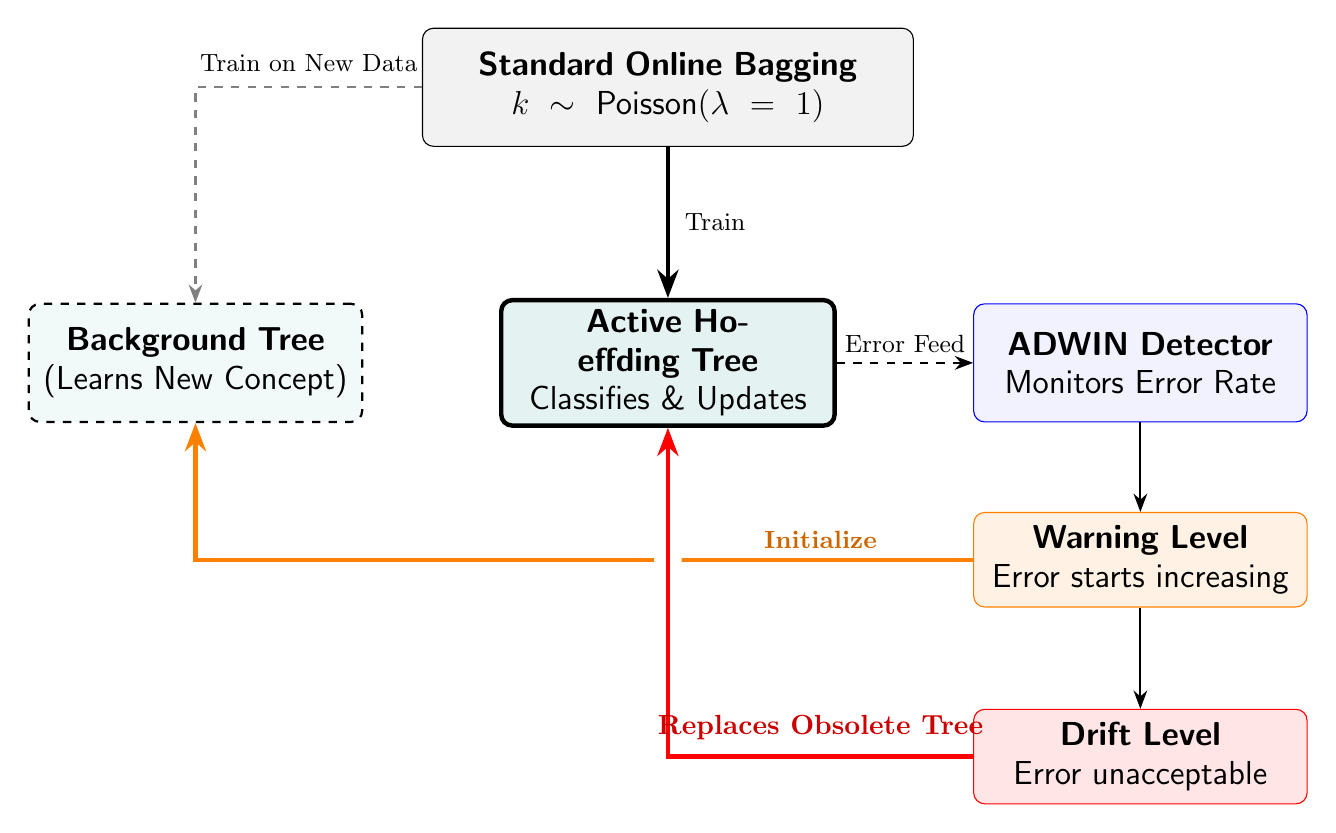
\begin{tikzpicture}[
    font=\sffamily\large,
    >=Stealth,
    block/.style={rectangle, draw, fill=gray!10, rounded corners, text width=6cm, text centered, minimum height=1.5cm},
    tree/.style={rectangle, draw=black, ultra thick, fill=teal!10, rounded corners, text width=4cm, text centered, minimum height=1.5cm},
    bg_tree/.style={rectangle, draw=black, thick, dashed, fill=teal!5, rounded corners, text width=4cm, text centered, minimum height=1.5cm},
    monitor/.style={rectangle, draw=blue, fill=blue!5, rounded corners, text width=4cm, text centered, minimum height=1.5cm},
    status/.style={rectangle, draw, rounded corners, text width=4cm, text centered, minimum height=1.2cm}
]

% Nodes
\node[block] (poisson) at (0, 0) {\textbf{Standard Online Bagging} \\ $k \sim \text{Poisson}(\lambda=1)$};
\node[tree] (tree) at (0, -3.5) {\textbf{Active Hoeffding Tree} \\ Classifies \& Updates};
\node[bg_tree] (bgtree) at (-6, -3.5) {\textbf{Background Tree} \\ (Learns New Concept)};
\node[monitor] (adwin) at (6, -3.5) {\textbf{ADWIN Detector} \\ Monitors Error Rate};

\node[status, draw=orange, fill=orange!10] (warning) at (6, -6) {\textbf{Warning Level} \\ Error starts increasing};
\node[status, draw=red, fill=red!10] (drift) at (6, -8.5) {\textbf{Drift Level} \\ Error unacceptable};

% Data Flow Arrows
\draw[->, ultra thick] (poisson.south) -- (tree.north) node[midway, right=2pt, font=\small] {Train};
\draw[->, dashed, thick, draw=gray] (poisson.west) -| (bgtree.north) node[near start, above=2pt, font=\small] {Train on New Data};

% Error & ADWIN Arrows
\draw[->, thick, dashed] (tree.east) -- (adwin.west) node[midway, above, font=\small] {Error Feed};
\draw[->, thick] (adwin.south) -- (warning.north);
\draw[->, thick] (warning.south) -- (drift.north);

% Warning Action (Orange)
\draw[ultra thick, draw=orange] (warning.west) -- (0, -6) node[midway, above, font=\small, text=orange!80!black] {\textbf{Initialize}};
\draw[->, ultra thick, draw=orange] (0, -6) -| (bgtree.south);

% White mask for clean crossing
\fill[white] (0, -6) circle (5pt);

% Drift Action (Red)
\draw[->, ultra thick, draw=red] (drift.west) -| (tree.south) node[near start, above=2pt, text=red!80!black, font=\bfseries] {Replaces Obsolete Tree};

\end{tikzpicture}
\end{document}
